% this file is called up by thesis.tex
% content in this file will be fed into the main document

%: ----------------------- name of chapter  -------------------------
\chapter{Weryfikacja rozwiązania} % top level followed by section, subsection


%: ----------------------- paths to graphics ------------------------

% change according to folder and file names
\ifpdf
    \graphicspath{{4/figures/PNG/}{4/figures/PDF/}{4/figures/}}
\else
    \graphicspath{{4/figures/EPS/}{4/figures/}}
\fi

%: ----------------------- contents from here ------------------------

Rozdział ten opisuje jak wybrany sposób integracji oraz powstały w ten sposób prototypowy system wpływa na łatwość tworzenia i efektywność aplikacji przetwarzających mowę. Proponowane przykładowe aplikacje to:
\begin{itemize}
	\item Automatyczne dyktando
	\item Lektor RSS
	\item Lektor SMS
	\item Konwerter plików graficznych do tekstowych
\end{itemize}
Każdej z proponowanych aplikacji poświęcono osobny podrozdział, w którym jest zdefiniowany przypadek użycia, przedstawione są wymagania funkcjonalne i niefunkcjonalne oraz przedstawiona jest weryfikacja podejścia.


\section{Automatyczne dyktando}
Jest to aplikacja web'owa umożliwiająca użytkownikowi ćwiczenie pisownii w różnych językach. Zasada działania jest bardzo prosta, użytkownik ładuje plik tekstowy lub graficzny na serwer oraz wybiera język docelowy, następnie zostaje przekierowany na stronę zawierającą formularz do pisania tekstu oraz odtwarzacz. Użytkownik słucha tekstu i zapisuje w polu tekstowym transkrypcję. W momencie w którym zatwierdzi formularz zostaje on przesłany na serwer i porównany z oryginalnym plikiem wejściowym, w efekcie użytkownik otrzymuje informację o ilości popełnionych błędów oraz o wyrazach które źle zapisał. 
\newpage
\subsection{Przypadek użycia}
\begin{figure}[!h]
	\centering
	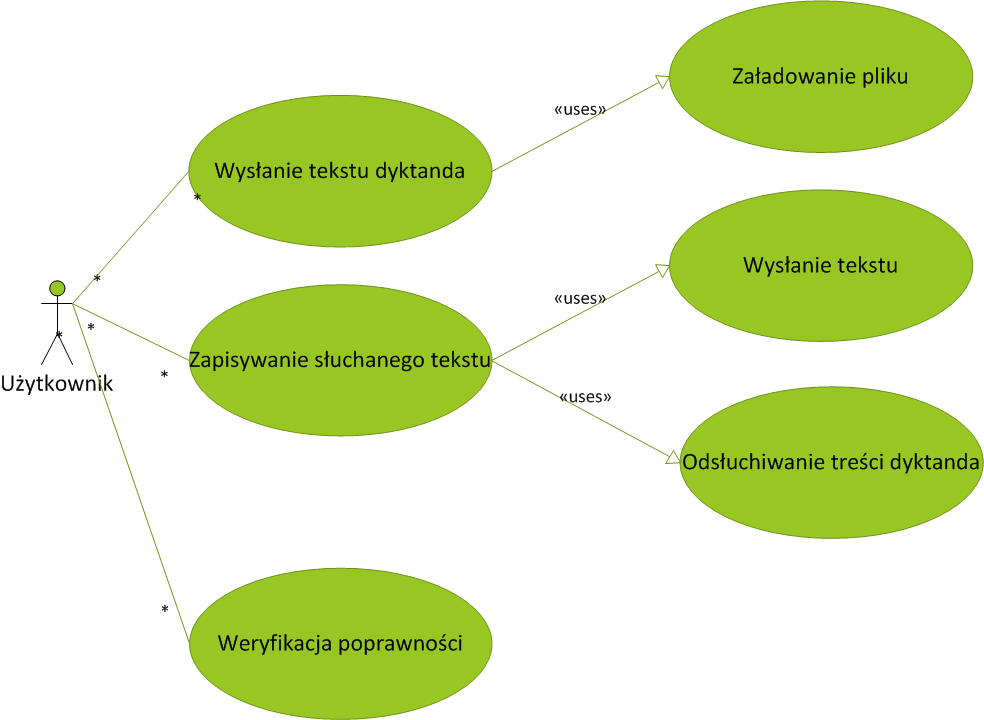
\includegraphics[scale=0.45]{useCaseDictando.png} 
	\caption{Przypadek użycia - Automatyczne dyktando }
\end{figure}

\subsection{Wymagania}
\subsubsection{Wymagania funkcjonalne}
\begin{enumerate}
	\item Obsługiwanie wielu języków
	\item Możliwość podania tekstu źródłowego
		\begin{enumerate}
			\item jako plik graficzny
			\item jako plik tekstowy, wysyłany na serwer
		\end{enumerate}
	\item Umożliwienie użytkownikowi odsłuchania wysłanego tekstu w wybranym przez niego języku
	\item Umożliwienie użytkownikowi wprowadzania tekstu jednocześnie z odsłuchiwaniem
	\item Wygenerowanie i wyświetlenie raportu o ilości błędów popełnionych przez użytkownika
\end{enumerate}

\subsubsection{Wymagania niefunkcjonalne}
\begin{enumerate}
	\item Bezpieczeństwo - użytkownik i tylko on powinien móc widzieć swoje wyniki
	\item Wydajność - dyktowanie tekstu powinno przebiegać płynnie, opóźnienia są niedozwolone ponieważ mogą dekoncentrować użytkownika
	\item Niezawodność - użytkownik powinien zawsze otrzymać wynik który jest poprawny, tzn. pokazuje dokładną ilość błędów popełnionych przez użytkownika
\end{enumerate}

\subsection{Weryfikacja podejścia}
Jak widać w powyższym podrozdziale wymagania stawiane przed aplikacją są precyzyjne i klarowne. Zastosowane podejście integracyjne sprawia, że stworzenie aplikacji spełniającej wymagania staje się proste. Zapewnienie obsługi wielu języków nie wymaga praktycznie żadnego nakładu pracy ze strony programisty aplikacji klienckiej. Jak zostało to opisane w rozdziale drugim, przy zastosowanym podejściu wystarczy wygenerować i przesłać plik xml z informacją dotyczącą języka docelowego, działa to niezależnie od języka w którym jest tekst wejściowy (pod warunkiem, że w pliku konfiguracyjnym ustawi się tag odpowiedzialny za serwis rozpoznający język). Podobnie przesłanie pliku graficznego, również wymaga tylko umieszczenia odpowiedniego tagu w pliku xml celem wywolania serwisu OCR. Jak łatwo zauważyć wygenerowanie i przesłanie pliku xml nie jest dużym wyzwaniem programistycznym.Widać to szczególnie gdyby porównać to z implementacją bez wykorzystania systemu opartego o rozwiązanie opisane w tej pracy. Musiałaby ona łączyć się z kilkoma zewnętrznymi serwisami, z których każdy prawdopodobnie miałby inny interfejs, konwertować różne formaty plików, obsługiwać błędy itd. Jedyną przewagą osobnej implementacji mogłabybyć szybkość działania, ale i tak różnica nie byłaby duża i sprowadzałaby się głównie do czasu potrzebnego na przesyłanie danych do i z systemu (oczywiście zakładając, że zarówno implementacja platformy jak i aplikacji korzystałaby z tych samych zewnętrznych serwisów). 
Jak widać, w tym przypadku, zastosowane podejście w sposób znaczący pozytywnie wpływa na łatwość i szybkość implementacji aplikacji klienckiej. \\

\section{Lektor RSS}
Jest to aplikacje web'owa której zadaniem jest odczytywanie wiadomości RSS ze źródeł podanych przez użytkownika, może on podać źródło przez specjalny formularz, załadować plik tekstowy zawierający adresy źródeł lub też wysłać plik w formacie graficznym z którego zostaną odczytane źródła. Niezależnie od użytej metody tekst wiadomości może być w dowolnym języku, podanym przez użytkownika lub też rozpoznanym przez system. Możliwe jest również przetłumaczenie wiadomości na język podany przez użytkownika i przeczytanie jej przez odpowiedniego lektora. Użytkownik ma również możliwość ustawienia co jaki czas ma następować sprawdzanie źródła celem znalezenia nowych wiadomości.	 

\subsection{Przypadek użycia}
\begin{figure}[!h]
	\centering
	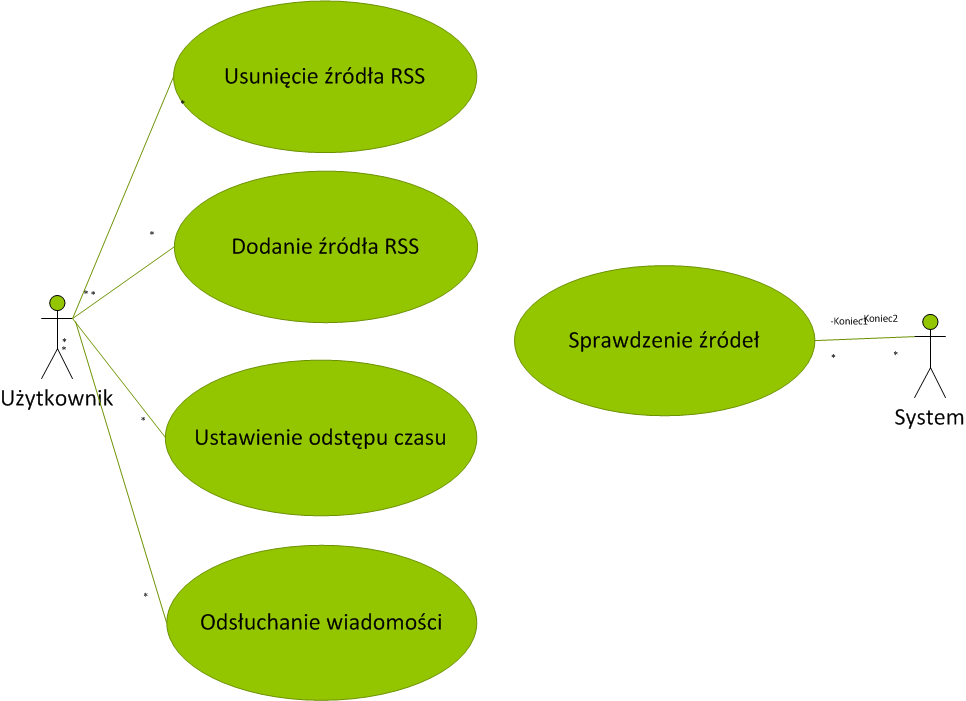
\includegraphics[scale=0.45]{useCaseRSS.png} 
	\caption{Przypadek użycia - LektorRSS}
\end{figure}

\subsection{Wymagania}
\subsubsection{Wymagania funkcjonalne}
\begin{enumerate}
	\item Możliwość dodania źródła RSS
	\item Możliwość usunięcia źródła RSS
	\item Obsługiwanie więcej niż jednego języka wiadomości
	\item Automatyczne sprawdzanie czy któreś ze źródeł nie zawiera nowej wiadomości
	\item Możliwość ustawienia odstępów czasowych pomiędzy sprawdzaniem przez system źródeł
	\item Automatyczne Odczytanie użytkownikowi nowych wiadomości (w przypadku istnienia) 
\end{enumerate}  
\subsubsection{Wymagania niefunkcjonalne}
\begin{enumerate}
	\item Bezpieczeństwo - użytkownik i tylko on powinien mieć dostęp do swojej listy źródeł RSS
	\item Niezawodność - system nie może pominąć żadnej wiadomości z listy źródeł zdefiniowanej przez użytkownika
	\item Szybkość - różnica czasu pomiędzy udostępnieniem nowej wiadomości w którymś ze źródeł a otrzymaniem jej przez użytkownika nie może przekraczać czasu pomiędzy sprawdzeniami w poszukiwaniu uaktualnień (czas ten ustawia użytkownik)
	\item Możliwość personalizacji - użytkownik powinien móc dodać dowolną ilość różnych źródeł, system powinien zapewnić ich niepowtarzalność(usuwać duplikaty)
\end{enumerate}

\subsection{Weryfikacja podejścia}
Tak jak w sekcji opisującej aplikację Automatyczne Dyktando wymagania przedstawione powyżej są jasne i klarowne. Po raz kolejny zastosowane podejście integracyjne sprawia, że napisanie aplikacji klienckiej, spełniającej wymagania przed nią stawiane jest proste. Dzięki użyciu ESB i oferowanych przez niego endpointów jest możliwe przerzucenie konieczności pobierania wiadomości ze źródeł RSS na stronę systemu. Podobnie jak w przypadku aplikacji opisanej wyżej zarówno rozpoznawanie języka, tłumaczenie czy generowanie mowy w odpowiednim języku nie stanowi dla programisty, autra aplikacji klienckiej żadnego problemu, wystarczającym jest wygenerowanie pliku xml zawierającego odpowiednie instrukcje. Implementacja podobnej, równie rozbudowanej aplikacji, bez wykorzystania systemu integrującego serwisy odpowiadające za przetwarzanie mowy byłaby bardzo trudna. Poza problemami podobnymi do tych jakie były opisane w przypadku Aumatycznego Dyktanda dochodzi jeszcze sprawa pobierania RSS'ów, ich parsowania itd. Pozostałe wymagania, takie jak bezpieczeństwo czy też konieczność przechowywania danych w bazie danych muszą być zaspokojone w ten sam sposób niezależnie od wykorzystania systemu. \\
W przypadku tej aplikacji również klarownym jest fakt, że użyte podejście bardzo upraszcza implementację.
 ----------------------------------------------------------------------------------------------------------------------------------------------------------------------
W celu weryfikacji prezentowanego rozwiązania 

Ten rodział opisuje wymagania które powinny być spełniane przez poszczególne, przykładowe aplikacje korzystające z serwisu UniversalSynthesizer. Podstawową funkcją serwisu jest udostępnianie usługi zamiany tekstu na mowę. Zaletą niniejszego systemu jest jego otwartość, możliwość wykorzystania innych niż proponowane syntezatorów mowy, łatwy dostęp przez web service, stosunkowo prosty sposób rozbudowy oraz możliwość jego wykorzystania do różnych celów na różnych platformach. Cechy te należy zademonstrować na przykładzie kilku prostych aplikacji, które muszą spełniać pewne jasno określone wymagania funkcjonalne i niefunkcjonalne opisane poniżej. 


Jest to prosta aplikacja dostępna dla użytkowników w formacie strony internetowej. Jej głównym celem jest wykorzystanie funkcji UniversalSynthesizer do dyktowania treści którą użytkownik zapisuje. Po odczytaniu całego tekstu i wysłaniu przez użytkownika formularza, jest on porównywany z tekstem oryginalnym w ten sposób może ćwiczyć swoją ortografie. Dużą zaletą jest to, że aplikacja ta nie jest ograniczona do jednego języka oraz fakt, że użytkownik sam podaje tekst.
\newpage
\subsubsection{Przypadki użycia} 
\begin{figure}[!h]
	\centering
	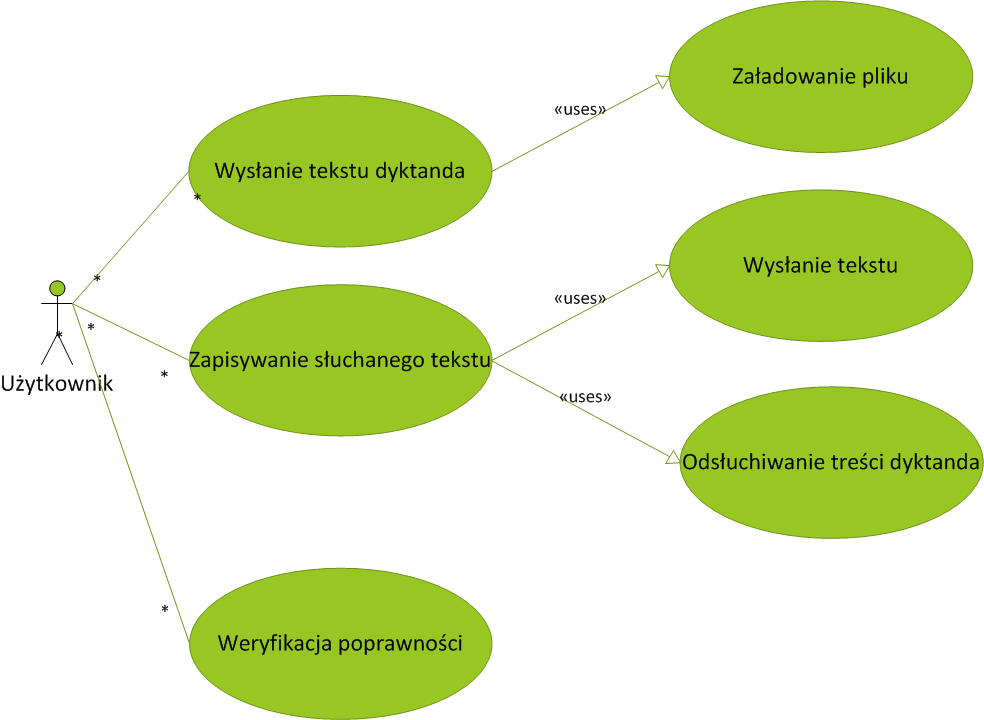
\includegraphics[scale=0.45]{useCaseDictando.png} 
	\caption{Przypadek użycia - Automatyczne dyktando }
\end{figure}

\subsubsection{Wymagania funkcjonalne}
\begin{enumerate}
	\item Obsługiwanie więcej niż jednego języka
		\begin{enumerate}
			\item polski
			\item angielski
			\item francuski
		\end{enumerate}
	\item Możliwość podania tekstu źródłowego
		\begin{enumerate}
			\item w formie tekstu wpisywanego na stronie
			\item jako plik tekstowy, wysyłany na serwer
		\end{enumerate}
	\item Umożliwienie użytkownikowi odsłuchania wysłanego tekstu w wybranym przez niego języku
	\item Umożliwienie użytkownikowi wprowadzania tekstu jednocześnie z odsłuchiwaniem
	\item Wygenerowanie i wyświetlenie raportu o ilości błędów popełnionych przez użytkownika
\end{enumerate}
\subsection{LektorRSS}
Jest to aplikacja webowa, które głównym celem jest odczytywanie użytkownikowi wiadomości RSS pobieranych z podanych przez niego źródeł. Należy zwrócić uwagę na duża zaletę tej aplikacji jaką jest fakt, że w zależności od języka wiadomości RSS jest ona odczytywana przez lektora odpowiedzialnego za ten język, oczywiście przy założeniu, że UniversalSynthesizer obłusguje język wiadomości.
\subsubsection{Przypadki użycia}


\subsubsection{Wymagania funkcjonalne}
\begin{enumerate}
	\item Możliwość dodania źródła RSS
	\item Możliwość usunięcia źródła RSS
	\item Obsługiwanie więcej niż jednego języka wiadomości
		\begin{enumerate}
			\item polski
			\item angielski
			\item francuski
		\end{enumerate}
		\item Automatyczne sprawdzanie czy któreś ze źródeł nie zawiera nowej wiadomości
	\item Możliwość ustawienia odstępów czasowych pomiędzy sprawdzaniem przez system źródeł
	\item Automatyczne Odczytanie użytkownikowi nowych wiadomości (w przypadku istnienia) 
\end{enumerate}  
\subsection{LektorsSMS}
Jest to aplikacja przeznaczona dla systemu operacyjnego Android. Jak nazwa wskazuje służy ona do automatycznego odczytywania wiadomości SMS zaraz po ich otrzymaniu. Jest bardzo przydatna w czasie jazdy samochodem, wiadomo, że używanie telefonu komórkowego jest zabronione z powodu bezpieczeństwa, tym bardziej, używanie rąk i skupianie wzrodku na odczytywanej wiadomości tekstowej jeszcze w większym stopniu niż rozmowa przez telefon prowadzi do odwrócenia uwagi kierowcy od sytuacji na drodze. Istnienie i użyteczność tej aplikacji pokazuje, że stworzony na potrzeby tej pracy serwis UniversalSynthesizer jest bardzo użyteczny, aplikacje mogące z niego korzystać mogą być tworzone na różne platformy.
\newpage
\subsubsection{Przypadki użycia}
\begin{figure}[!h]
	\centering
	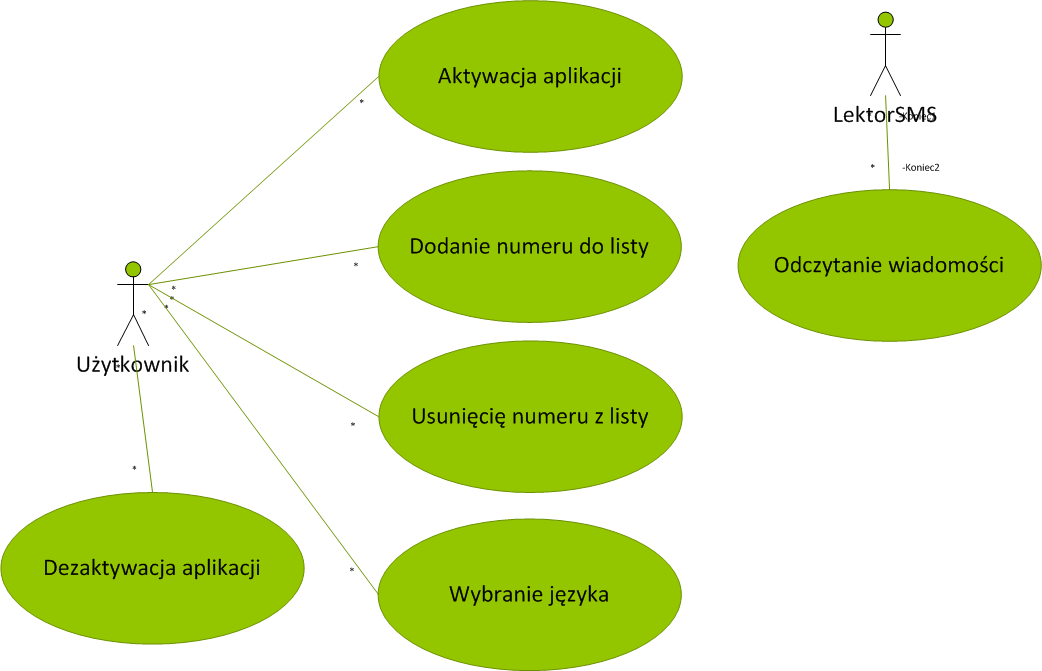
\includegraphics[scale=0.45]{useCaseLektorSMS.png} 
	\caption{Przypadek użycia - LektorRSS}
\end{figure}

\subsubsection{Wymagania funkcjonalne}
\begin{enumerate}
	\item Możliwość aktywacji i dezaktywacji aplikacji
	\item Możliwość ustawienia języka w którym będzie odczytywana treść wiadomości
	\item Możliwość filtrowania obsługiwanych wiadomości SMS po numerach nadawców 
	\item Obsługiwanie więcej niż jednego języka wiadomości
		\begin{enumerate}
			\item polski
			\item angielski
			\item francuski
		\end{enumerate}
	\item Automatyczne odczytywanie otrzymanych wiadomości
\end{enumerate}

\section{Wymagania niefunkcjonalne}
\subsection{Automatyczne dyktando}
\subsubsection{Wymagania niefunkcjonalne}
\begin{enumerate}
	\item Bezpieczeństwo - użytkownik i tylko on powinien móc widzieć swoje wyniki
	\item Wydajność - dyktowanie tekstu powinno przebiegać płynnie
	\item Niezawodność - użytkownik powinien zawsze otrzymać wynik który jest poprawny i jest jego wynikiem
\end{enumerate}
\subsection{Lektor RSS}

\subsection{LektorsSMS}
\begin{enumerate}
	\item Bezpieczeństwo - dostęp do apikacji musi być chroniony hasłem
	\item Użyteczność - poprawne działanie na dowolnym urządzenie z systemem Android posiadającym dostęp do sieci
	\item Wydajność - musi działać na starszych i słabszych telefonach
\end{enumerate}

% ---------------------------------------------------------------------------
%: ----------------------- end of thesis sub-document ------------------------
% ---------------------------------------------------------------------------

